\documentclass[letterpaper, 12pt]{article}
\usepackage{graphicx}
\graphicspath{{Figures/}{./}}
\usepackage{apacite}
\usepackage{amsmath}
\usepackage{amssymb}
\usepackage{amsthm}
\usepackage{indentfirst}
\usepackage[justification=centering]{caption}
\usepackage{float}

\title{MATHEMATICS ANALYSIS AND APPROACHES HL
\\
Producing the IB Logo with the Fourier Series}
\author{}
\date{}

\begin{document}
\nocite{*}

\maketitle
\begin{center}
    Candidate Code:
    \\
    Session: May 2024
    \\
    Page Count:
\end{center}
\newpage

\tableofcontents
\newpage

\section{Rationale}

I have shown interest in visual arts done through the means of software,
with particular experience in 3D modelling and animation in Blender
and Cinema 4D.

I never was experienced with drawing, therefore producing digital art
on a 2D plane using artistic skill was not of interest to me. However,
something that I came across online was the use of the Fourier Series
in order to produce vector art, which instantly intrigued me.

While vector art files such as those with the file extension ".svg" relate
to mathematics in the sense that it contains multiple graphed mathematical
relationships in order to produce an image, the method of using the Fourier
Series to produce similar art is more mathematically intriguing, as it
proves use just one expression to produce the same result done by the numerous mathematical
relationships.


\section{Aim}

The objective of this investigation is to link Fourier series with
complex numbers to create a single series that is capable
of reproducing the IB logo on the Argand plane.

\section{Plan of Action}

This exploration focuses on the following areas of math:
\begin{itemize}
    \item Integral Calculus
    \item Series
    \item Trigonometry
    \item Complex Analysis
    \item Vectors
\end{itemize}

\section{Background Information}

\subsection{Basics behind the Fourier Series}

A periodic function is one where the output for a particular input equals to
the output for the sum of the same input and the value of the function's period.
This can be represented mathematically as:
\begin{align*}
     & f(x) = f(x + P)
    \\
     & \text{where } P = \text{ the period of the function}
\end{align*}

The sine wave is widely known for being a periodic function for the ease of graphing
a sinusoidal wave. However, there are periodic functions that are difficult to
graph with an algebraic expression, such as one that alternates between
1 and -1 or one that is shaped as a zig-zag.

This is the motivation behind the Fourier Series, which is to be able to represent
period functions that normally can't be represented by an algebraic function.

The idea behind the Fourier Series is to take an infinite sum of varying sinusoidal
functions such that a desired periodic function is produced.

\begin{figure}[H]
    \centering
    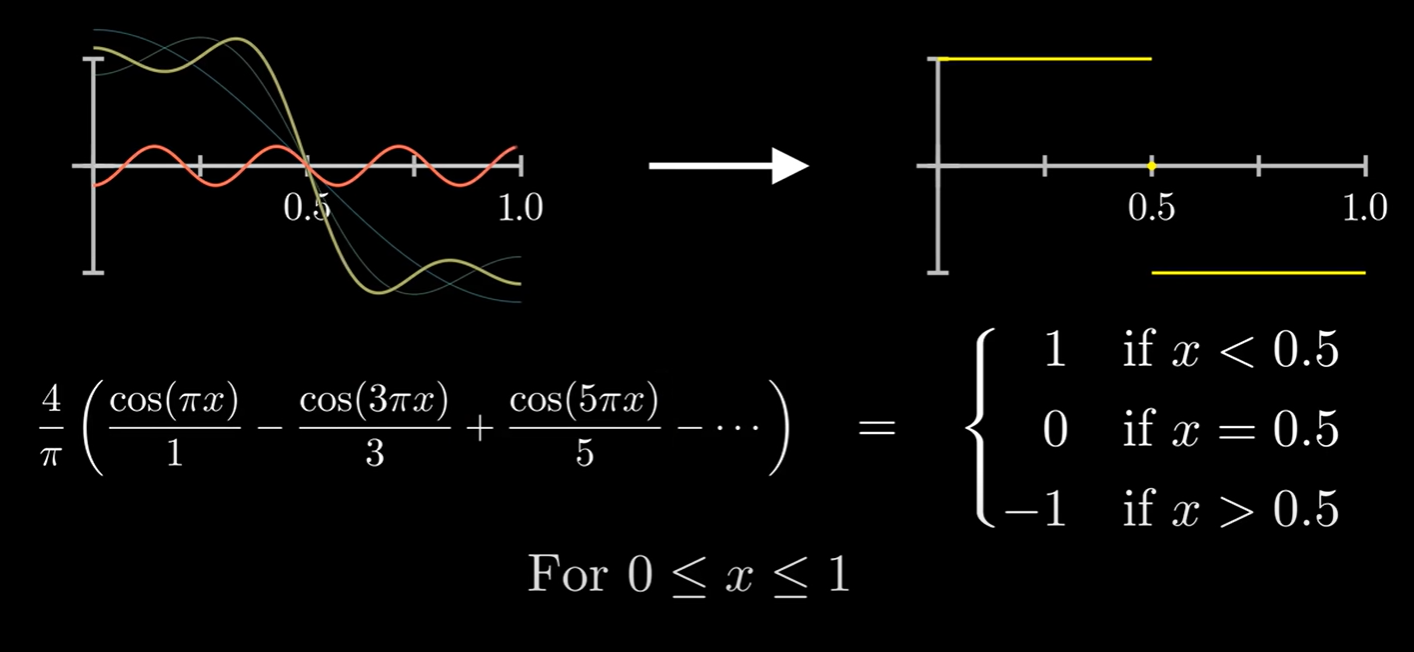
\includegraphics[width=\textwidth]{fourier_basic_visual.png}
    \caption{Visualization of the mechanism of the Fourier Series \protect\cite{sandersonWhatFourierSeries2019}. The yellow line is the periodic function resulting from the previous iteration, the red line is the sinusoidal function to be added in the next iteration.}
    \label{fig:fourier_visual}
\end{figure}

A general formula for representing a periodic function as a Fourier Series with a
period of \(2\pi\) is:
\[
    f(t) = \frac{a_0}{2} + \sum_{n = 1}^{\infty} a_n \cos{nt} + \sum_{n=1}^{\infty} b_n\sin{nt}
\]

\subsection{Fundamental application to draw on the Cartesian Plane}

\subsection{Rotating vectors on the Argand Plane}

\subsection{Enriched application to draw on the Argand Plane}


\bibliographystyle{apacite}
\bibliography{IB_MATH_IA.bib}

\end{document}